% !Mode:: "TeX:UTF-8"
\RequirePackage[l2tabu, orthodox]{nag}
%\documentclass[a4paper,twocolumn, 11pt]{article}
\documentclass[a4paper,11pt]{article}
%%%% FILL THESE OUT %%%%
\newcommand{\mySubject}{Principles of Computer System Design}
\newcommand{\myLocation}{DIKU}
\newcommand{\myAssignment}{Assignment 1}
\newcommand{\myAuthor}{Martin Grunbaum (martin@itsolveonline.net)}
\newcommand{\myShortAuthor}{Martin G.}

%%%% PACKAGES %%%%
\usepackage[T1]{fontenc}
\usepackage{amsmath, amssymb, amsthm}
\usepackage[table,usenames,dvipsnames]{xcolor}
\usepackage[utf8]{inputenc}
\usepackage[english]{babel}
\usepackage{placeins}
\usepackage{graphicx}
\usepackage{url}
\usepackage[colorlinks=true]{hyperref}
\usepackage{fancyhdr}
\usepackage{lastpage}
\usepackage{paralist}
\usepackage{parskip}
\usepackage{algorithmicx}
\usepackage{algpseudocode}
\usepackage{fullpage}
\usepackage{lmodern}
\usepackage[nounderscore]{syntax}
\usepackage{lipsum}
\usepackage{multicol}
\usepackage{float}
\usepackage[framemethod=TikZ]{mdframed}
\usepackage{booktabs}
\usepackage{cleveref}

%%%% PACKAGE SETTINGS & GENERAL ALTERATIONS %%%%

% Page margins
\renewcommand{\headrulewidth}{0in}
\setlength\headsep{40pt}
\setlength\headheight{20pt}
\addtolength{\textheight}{-20pt}
\setlength{\columnsep}{20pt}

% Boxed floats
\floatstyle{boxed}
\restylefloat{figure}

% MD Frames
\mdfdefinestyle{stubFrame}{%
    linecolor=red,
    linewidth=3pt,
    leftmargin=1cm,
    innerleftmargin=20pt,
    innerrightmargin=20pt,
    rightmargin=1cm,
    topline=false,
    bottomline=false}
\mdfsetup{skipabove=\topskip,skipbelow=\topskip}

\mdfdefinestyle{theoremstyle}{%
    linecolor=red,linewidth=2pt,%
    frametitlerule=true,%
    frametitlebackgroundcolor=gray!20,
    innertopmargin=\topskip,
}

% \maketitle-related
\title{\mySubject}
\author{\myAuthor}

% Fancy header
\pagestyle{fancy}
\lhead{\footnotesize \myShortAuthor\\\ }
\chead{\footnotesize\mySubject\\\myAssignment}
\rhead{\footnotesize\myLocation\\\today}
\cfoot{\thepage/\pageref*{LastPage}}

\begin{document}
    \maketitle
\section{Serializability \& Locking}
Concurrency introduces a number of problems that
must be either partially or completely solved, depending on the desired
trade-off between correctness and speed. Two-phase locking protocols are
aimed at providing certain guarantees, that aid in the concurrent execution of
data reads and writes. There are a myriad of different ones, but this report
does not dive into the differences. We consider two specific \textbf{transaction schedules} 
here, shown below.

\begin{table}[!htb]
    \begin{minipage}{.5\linewidth}
        \caption*{Schedule 1}
        \begin{tabular}{c|c|c}
            \textit{T1} & \textit{T2} & \textit{T3} \\ \hline
            R(X) & & \\
            & W(Z) & \\
            & W(X) & \\
            & C & \\
            & & \\
            & & R(Z) \\
            & & R(Y) \\
            & & C \\
            W(Y) & & \\
            C & & \\
        \end{tabular}
    \end{minipage}
    \begin{minipage}{.5\linewidth}
        \caption*{Schedule 2}
        \begin{tabular}{c|c|c}
            \textit{T1} & \textit{T2} & \textit{T3} \\ \hline
            R(X) & & \\
            & & W(Z) \\
            & & C \\
            & R(Z) & \\
            W(Y) & & \\
            C & & \\
            & W(X) & \\
            & W(Y) & \\
            & C &
        \end{tabular}
    \end{minipage}
\end{table}
\begin{figure}[!h]
    \begin{minipage}{.5\linewidth}
        \caption{Precedence graph for Schedule 1\label{fig:sched1_prec}}
        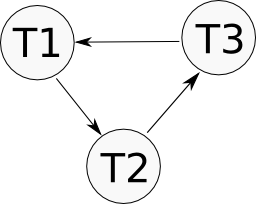
\includegraphics[scale=0.75]{images/sched1.png}
    \end{minipage}
    \begin{minipage}{.5\linewidth}
        \caption{Precedence graph for Schedule 2\label{fig:sched2_prec}}
        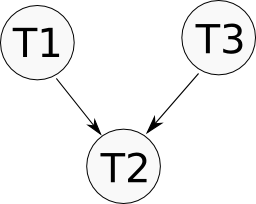
\includegraphics[scale=0.75]{images/sched2.png}
    \end{minipage}
\end{figure}

\FloatBarrier
The schedules should be read top-down, each schedule consisting of one or more
transactions occuring concurrently. Each transaction ends with a
\textbf{C}ommit. Figures~\ref{fig:sched1_prec} and~\ref{fig:sched2_prec} show
the precedence graphs for each of the schedules, which help shed light on which
transactions cause conflicts with other transactions. An arrow from one
transaction to another indicates that the source transaction performs an action
before the target transaction, that would cause a conflict. A cyclic graph in
such an instance is bad news, as such a graph is not
\textbf{conflict-serializable} through e.g.\ strict two-phase locking.


\subsection{Schedule 1}

As can be seen, Schedule 1 has a cyclic precedence graph, leading to a schedule that is
\textbf{not} \textit{conflict-serializable}. An acyclic graph indicates that we
can select some topological sorting over the precedence graph to generate a
serial schedule. In particular for Schedule 1, T1's read on X will cause T2 to
be unable to obtain a write-lock on X, which prevents T2 from committing. At
that time, however, T2 has also obtained a write-lock on Z, which T3 needs
before \textbf{it} can commit. Schedule 1 could \textbf{not} have been generated
by strict two-phase locking, as strict two-phase locking guarantees an acyclic
precedence graph that is \textit{conflict-serializable}.

\subsection{Schedule 2}
Schedule 2 has an acyclic precedence graph, and \textbf{is}
\textit{conflict-serializable}. A version of Schedule 2 with read and write
locks injected can be seen in Table~\ref{tbl:sched2}

\begin{table}[!htb]
    \begin{tabular}{c|c|c}
        \textit{T1} & \textit{T2} & \textit{T3} \\ \hline
        S(X) & & \\
        R(X) & & \\
        & & X(Z) \\
        & & W(Z) \\
        & & C \\
        & S(Z) & \\
        & R(Z) & \\
        X(Y) & & \\
        W(Y) & & \\
        C & & \\
        & X(X) & \\
        & W(X) & \\
        & X(Y) & \\
        & W(Y) & \\
        & C & 
    \end{tabular}
    \caption{Schedule 2 with read/write locks injected.\label{tbl:sched2}}
\end{table}

\section{Optimistic Concurrency Control}
In strict concurrency control, we attempt to prevent bad behavior by being very
thorough about the way instructions are (re-)organized. Optimistic concurrency
control realizes the belief that in some cases, the overhead introduced by doing
so may be greater than the benefit. In some situations conflicts are very rare
and so a different approach can perhaps be taken instead. In optimistic
concurrency control transactions are considered a three-phase process:
\begin{inparaenum}[1)]
\item Read phase.
\item Validation phase.
\item Write phase.
\end{inparaenum}
If a transaction passes the validation phase, it can be safely written. Doing so
requires upholding three validation conditions, as pr. \cite[p. 91]{pcsd}.
Below, we consider three different scenarios where each transaction has a set of
reads and writes, and answer the question: Should the third transaction,
\texttt{T3}, be allowed to commit or be rolled back? In all of the scenarios it
is assumed that \texttt{T1} and \texttt{T2} both passed validation.

\subsection{Scenario 1}
From the assignment:

\begin{verbatim}
T1: RS(T1) = {1, 2, 3}, WS(T1) = {3},
    T1 completes before T3 starts.
T2: RS(T2) = {2, 3, 4}, WS(T2) = {4, 5},
    T2 completes before T3 begins with its Write phase.
T3: RS(T3) = {3, 4, 6}, WS(T3) = {3},
    allow T3 to commit or roll back?
\end{verbatim}

As \texttt{T1} completes before \texttt{T3} begins, there are no potential
conflicts between those two transactions (criterion 1). \texttt{T2} completes
before \texttt{T3}'s Write phase, but \texttt{T2} writes to \textbf{4} which
\texttt{T3} reads. \texttt{T3} should be rolled back because of violating
criterion 2 with regards to object \textbf{4}.

\subsection{Scenario 2}
From the assignment:

\begin{verbatim}
T1: RS(T1) = {1, 2, 3}, WS(T1) = {3},
    T1 completes before T3 begins with its Write phase.
T2: RS(T2) = {5, 6, 7}, WS(T2) = {8},
    T2 completes Read phase before T3 does.
T3: RS(T3) = {3, 4, 5, 6, 7}, WS(T3) = {3},
    allow commit or roll back?
\end{verbatim}

\texttt{T1} completes before \texttt{T3}'s Write phase, and \texttt{T1} writes
to object \textbf{3} which \texttt{T3} reads (criterion 2). Also, \texttt{T2}
completes reading before T3 does but shares reads on objects \textbf{5, 6} and
\textbf{7} with \texttt{T3} (criterion 3). \texttt{T3} should thus be rolled
back.

\subsection{Scenario 3}
From the assignment:

\begin{verbatim}
T1: RS(T1) = {2, 3, 4, 5}, WS(T1) = {4},
    T1 completes before T3 begins with its Write phase.
T2: RS(T2) = {6, 7, 8}, WS(T2) = {6},
    T2 completes before T3 begins with its Write phase.
T3: RS(T3) = {2, 3, 5, 7, 8}, WS(T3) = {7, 8},
    allow commit or roll back?
\end{verbatim}

\texttt{T1} completes before \texttt{T3}'s Write phase and does not write to any
object that \texttt{T3} reads. \texttt{T2} completes before \texttt{T3}'s Write
phase and does not write to any object that \texttt{T3} reads. As such,
\texttt{T3} passes the validation phase and can be committed.

\section{Discussion on the Concurrent Implementation of the Bookstore}
The locking protocol implemented in the codebase makes use of a so-called
re-entrant read/write locking solution. The lock keeps track of callers on a
Thread-basis, and callers can request several subsequent read and/or write
locks, hence the re-entrant nature of the lock. Writes are prioritized above
reads when both are queued and a caller that holds a read lock can request a
write lock if needed, and vice versa.

The locking scheme is similar to strict two-phase locking, in that it entertains
a notion of a shared lock (read lock) and an exclusive lock (write lock). A
caller that holds an exclusive lock can obtain the shared lock as well, and can
also go from being the sole holder of the shared lock to also holding the
exclusive lock. However, once an exclusive lock has been established then no
other threads can establish a shared or exclusive lock until it is released.
While the code itself makes no guarantee/requirement for it, the bookstore
releases all locks at the end of use as per strict two-phase locking.

The logic that governs whether a read or write lock can be established is shown
below, copied verbatim from the source code as it is quite readable. A thread
requesting a read or write lock will block while waiting for the appropriate
method to return true:

\begin{verbatim}
private boolean couldWrite(Thread caller) {
    if(this.isOnlyReader(caller)) return true;
    if(this.hasAnyReaders()) return false;
    if(!this.hasWriter()) return true;
    if(!this.isWriter(caller)) return false;
    return true;
}

private boolean couldRead(Thread caller) {
    if(this.isWriter(caller)) return true;
    if(this.hasWriter()) return false;
    if(this.isReader(caller)) return true;
    if(this.hasWriteRequests()) return false;
    return true;
}
\end{verbatim}

The protocol is vulnerable to deadlocks, if e.g.\ thread A locks resource
\textbf{X}, thread B locks resource \textbf{Y} and they both attempt to lock the
object the other thread is holding as the next step in their process. There are
several potential ways to avoid this, such as a waits-for graph or timeouts. A
timeout-based solution might keep track of the waiting time during attempting to
acquire a lock, and may stop trying after a (semi-randomized) period of time,
releasing all other locks currently held at the same time.

There are still scalability issues in the current solution, as the model itself
is not distributed across multiple machines. So you can scale vertically and
increase the specs of the machine that runs the 'database model', but horizontal
scaling is not possible as-is. Switching to an RDBMS or another real
database-based solution would help with scalability issues, but even with modern
databases scalability is \textbf{always} a difficult issue that warrants
significant amounts of effort dedicated to optimizing throughput, concurrency,
scalability, reliability and such through master/master-replication,
master/slave-replication, map-reduce paradigms and a host of other interesting
technologies and designs. There are, in general, no infinitely scalable services
in practice.

The protocol implemented has very low overhead, as it is used to lock the entire
book map. This is both good and bad: It means keeping track of what is locked is
incredibly easy and requires a single map of readers and a single reference to a
potential writing thread, but it also means that concurrency is not as
pronounced as it could be, if I instead had opted to lock on e.g.\ individual
books. The provided solution does good work towards providing a concurrent
solution and especially the methods which first initially validate input against
the book store model benefit greatly from only (mostly) having to read-lock that
portion of the method, freeing up others to still perform writes.

\end{document}
